{}\documentclass[letterpaper,
compress,
xcolor=x11names,
%draft,
]{beamer}
% Package imports
\usepackage{mathtools} % imports `amsmath'
\DeclareMathOperator{\sech}{sech}
\usepackage{amssymb}
\usepackage{fixltx2e}
\usepackage{lmodern}
\usepackage{movie15}
%\usepackage{media9}
\usepackage{microtype}
\usepackage{animate}
\usepackage{subcaption}
\captionsetup{compatibility=false}

% I just did this
\usepackage[english]{babel}
\usepackage[utf8]{inputenc}
\usepackage{amsmath}
\usepackage{graphicx}
\usepackage[colorinlistoftodos]{todonotes}
\usepackage{tikz}
\usetikzlibrary{tikzmark}
\usepackage{array}
\usepackage{layout}
\usepackage{multicol}
\usepackage{multirow}
\usepackage{booktabs}
\usepackage{url}
\usepackage{hhline}
%I just did this

% `beamer' configuration
\usefonttheme{professionalfonts}
\useoutertheme[subsection=false,]{miniframes}
\setbeamercolor*{alerted text}{fg=red}
\setbeamercolor*{example text}{fg=black}
\definecolor{CSU_green}{RGB}{30, 70, 43}
\definecolor{CSU_gold}{RGB}{200, 195, 114}
\setbeamercolor*{lower separation line head}{bg=CSU_gold}
\setbeamercolor*{section in head/foot}{fg=white,bg=CSU_green}
\setbeamercolor*{subsection in head/foot}{bg=white}
\setbeamercolor*{upper separation line head}{bg=CSU_gold}
\setbeamercolor*{page number in head/foot}{fg=CSU_green}
\setbeamercolor*{normal text}{fg=black,bg=white}
\setbeamercolor*{palette tertiary}{fg=black,bg=black!10}
\setbeamercolor*{palette quaternary}{fg=black,bg=black!10}
\setbeamercolor*{structure}{fg=black}
\setbeamerfont{frametitle}{shape=\scshape}
\setbeamerfont{institute}{shape=\scshape}
\setbeamerfont{section in head/foot}{shape=\scshape}
\setbeamerfont{subsection in head/foot}{shape=\scshape}
\setbeamertemplate{bibliography item}{}
\setbeamertemplate{itemize items}[ball]
\setbeamertemplate{navigation symbols}{}
\setbeamertemplate{footline}[frame number]
\usetikzlibrary{calc,arrows}
\graphicspath{{graphics/}{graphics/movies/}{graphics/images/}}
\usepackage{remreset}                  % hack to display beamer navigation
\makeatletter                          % circles even if not declaring
\@removefromreset{subsection}{section} % subsections
\makeatother                           % see: http://tex.stackexchange.com/a/2078
\setcounter{subsection}{1}             % see: https://bitbucket.org/rivanvx/beamer/issue/218

% `biblatex' configuration
\usepackage[backend=biber,
style=authortitle-comp,
]{biblatex}
\addbibresource{presentation.bib}

% `enumitem' configuration
\usepackage{enumitem}
\setlist[itemize,1]{label=\usebeamertemplate{itemize item}}
\setlist[itemize,2]{label=\usebeamertemplate{itemize subitem}}
\setlist[itemize,3]{label=\usebeamertemplate{itemize subsubitem}}
\DeclareMathOperator{\sinc}{sinc}


% `graphicx' configuration
\usepackage{graphicx}
\begin{document}
	\title{Logic and Loops}
	%\subtitle{MATH-151:  Mathematical Algorithms in Matlab}
	\author{MATH-151:  Mathematical Algorithms in Matlab}
	\date[202X]{August 28, 2023}
	\titlegraphic{
\includegraphics[height = 3cm]{CSU_Ram_Logo.jpg}}



%%%%%%%%%%%%%%%%%%%%%%%%%%%%%%%%%%%%%%%%%%%%%%%%%%%%%%

\begin{frame}
\titlepage
\end{frame}
%%%%%%%%%%%%%%%%%%%%%%%%%%%%%%%%%%%%%%%%%%%%%%%%%%%%%%%%%
\section{Logic}

\begin{frame}{Formal Logic Statements}
	\footnotesize
	\begin{itemize}
		\item In general, a \textbf{logical statement} is a declarative sentence to which one (and only one) of the terms ``true" or ``false" can be \underline{meaningfully applied}
		\begin{itemize}
			\item Air Bud is a dog that plays basketball. (True statement!)
			\item $\pi$ = 3 (False statement!)
			\item This statement is false. (Neither! Can't meaningfully apply true or false)
			\item Let's go Air Bud! (This isn't a statement, not declarative) 
		\end{itemize}
		\item<2-> Because computers ``think" in 1s and 0s, logical statements are very useful in computing.
		\begin{itemize}
			\item 1 means true. 0 means false.
		\end{itemize}
		\item<2-> Logical statements allows us to turn parts of our code ``on" and ``off" using control statements
	\end{itemize}
	\begin{center}
		\onslide<2->{
\includegraphics[height = 2cm]{ones_n_zeros.jpg}}
	\end{center}
\end{frame}

%%%%%%%%%%%%%%%%%%%%%%%%%%%%%%%%%%%%%%%%%%%%%%%%%%%%%%%%%

\begin{frame}{Logical Statements in Code}
	\footnotesize
	Great! We now know what a logical statement is, but how can we make our logical statements in Matlab? The most common ones we will use are \textbf{relational statements}
	\begin{columns}
		\begin{column}{0.7\linewidth}
			\begin{itemize}
				\item<2-> Equality (\texttt{==})
				\begin{itemize}
					\item This returns true if the values on both sides of the \texttt{==} are the same, and false if not
					\item Example: We can see if a value is even by seeing if dividing by two gives us an integer\\
					\centering{\texttt{x/2 == round(x/2)}}	
				\end{itemize}
				\item<3-> Inequalities (\texttt{\textgreater, \textgreater=, \textless, \textless=})
				\begin{itemize}
					\item Checks how one value relates to another
					\item Example: Check if grade is an A \\
					\centering{\texttt{score \textgreater= 93}}
				\end{itemize}
				\item<4-> Not equality \texttt{\url{~}=} 
				\begin{itemize}
					\item This is the opposite of equality.
					\item Example: Value is odd if dividing by two is not an integer \\
					\centering{\texttt{x/2 \url{~}= round(x/2)}}
				\end{itemize}
			\end{itemize}
		\end{column}
		\begin{column}{0.25\linewidth}
			\begin{center}
				\onslide<2->{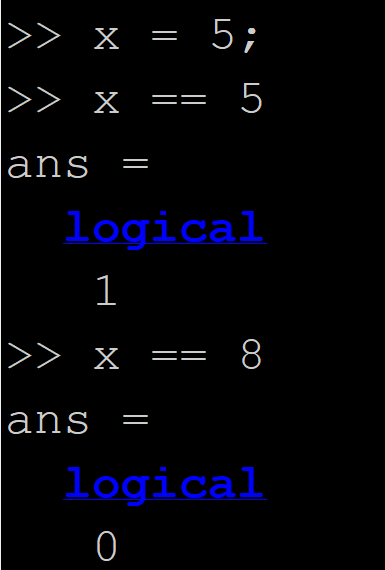
\includegraphics[height = 2cm]{equality_example.png}} \\
				\onslide<3->{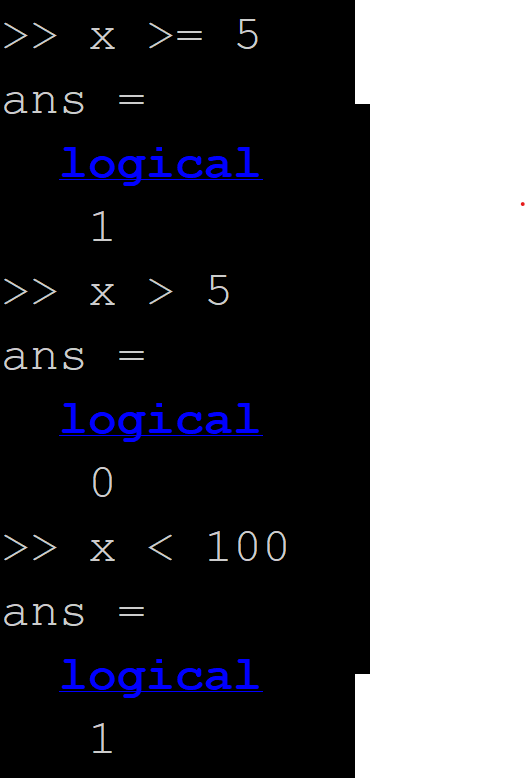
\includegraphics[height = 2cm]{inequality_example.png}} \\
				\onslide<4->{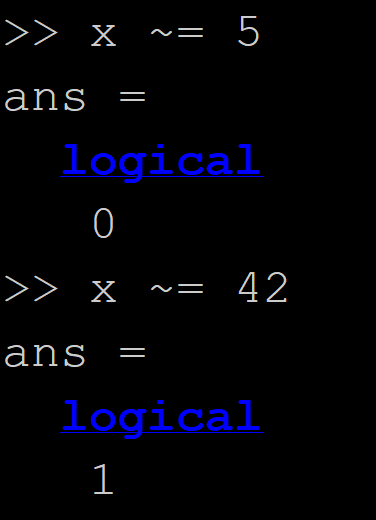
\includegraphics[height = 2cm]{notequality_example.png}}
			\end{center}
		\end{column}
	\end{columns}
\end{frame}

%%%%%%%%%%%%%%%%%%%%%%%%%%%%%%%%%%%%%%%%%%%%%%%%%%%%%%%%%

\begin{frame}{If ... Else .. Statements}
	\footnotesize
	\begin{itemize}
		\item Sometimes in life we have contingencies
		\begin{itemize}
			\item If it is raining, bring an umbrella. Else, don't bring an umbrella.
		\end{itemize}
		\item<2-> Algorithms have these as well! Consider the median
		\begin{itemize}
			\item If there is an odd number of data values, take the center value
			\item If there is an even number of data values, average the center two. 
		\end{itemize}
		\item<3-> \texttt{if ... else ...} statements in code allow us to do this. See our example for the median
		\begin{center}
			\onslide<3->{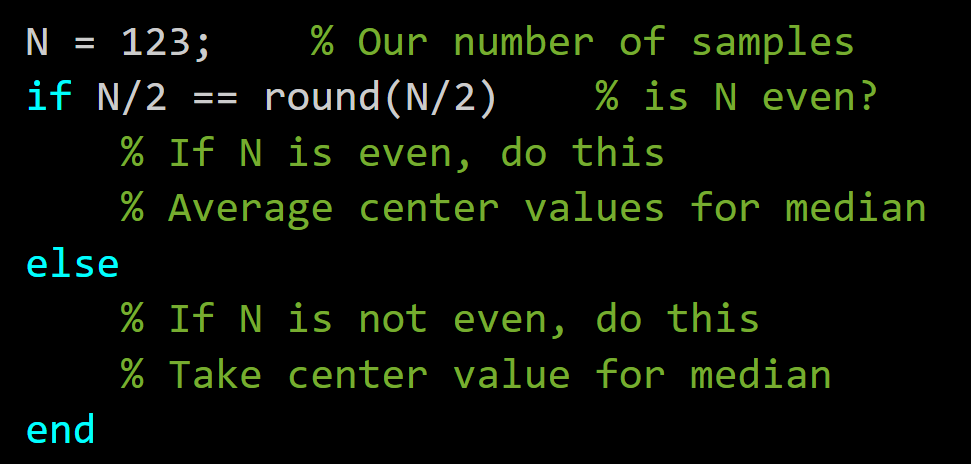
\includegraphics[width = 5cm]{median_if_example.png}}
		\end{center}
	\end{itemize}
\end{frame}

%%%%%%%%%%%%%%%%%%%%%%%%%%%%%%%%%%%%%%%%%%%%%%%%%%%%%%%%%
\begin{frame}{Elseif Statements}
	\footnotesize
	\begin{itemize}
		\item In many cases the decisions are more than just two options!
		\begin{itemize}
			\item If it is morning, eat breakfast. If it is noon, eat lunch. If it is evening, eat dinner. Otherwise, don't eat a meal.
		\end{itemize}
		\item<2-> We can add additional conditions between our \texttt{if} and \texttt{else} using \texttt{elseif}.
		\item<2-> For example my vehicle code controlled differently based on range from object, and whether or not it has detected the object yet
		\begin{center}
			\onslide<2->{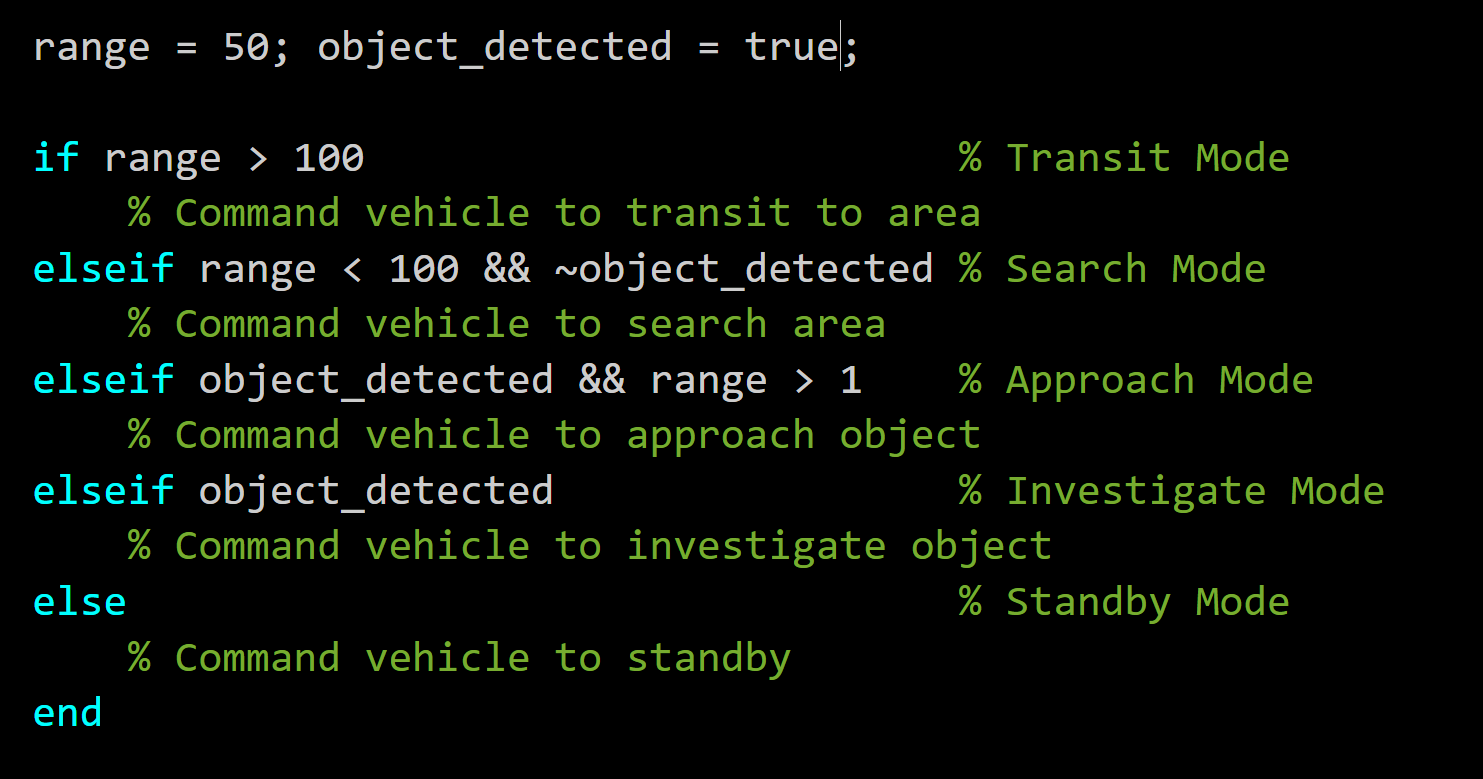
\includegraphics[width = 5cm]{elseif_example.png}}
		\end{center}
		\item<3-> The computer starts at the \texttt{if} statement, and works its way down the \texttt{elseif} statements until one of them are true.
	\end{itemize}
\end{frame}
%%%%%%%%%%%%%%%%%%%%%%%%%%%%%%%%%%%%%%%%%%%%%%%%%%%%%%%%%

\begin{frame}{Boolean Operators}
	\footnotesize
	\textbf{Boolean operators} are functions allowing us to link together multiple logical statements into one
	\begin{columns}
		\begin{column}{0.5\linewidth}
			\begin{itemize}
				\item<2-> and (\texttt{p \&\& q}) \\
				\begin{tabular}{c  c || c | c }
					\multicolumn{2}{c}{\multirow{2}{*}{\texttt{p \&\& q}}} & \multicolumn{2}{c}{\texttt{p}} \\
					& & 1 & 0 \\
					\hhline{~=||=|=}
					\multirow{2}{*}{\texttt{q}} & 1 & 1 & 0 \\
					\cline{2-4}
					 & 0 & 0 & 0 \\
				\end{tabular}
				\vspace{0.5cm}
				\item<4-> xor (\texttt{xor(p,q)})
				\begin{tabular}{c  c || c | c }
					\multicolumn{2}{c}{\multirow{2}{*}{\texttt{xor(p,q)}}} & \multicolumn{2}{c}{\texttt{p}} \\
					& & 1 & 0 \\
					\hhline{~=||=|=}
					\multirow{2}{*}{\texttt{q}} & 1 & 0 & 1 \\
					\cline{2-4}
					& 0 & 1 & 0 \\
				\end{tabular}	
			\end{itemize}
		\end{column}
		\begin{column}{0.5\linewidth}
			\begin{itemize}
				\item<3-> or (\texttt{p || q}) \\
				\begin{tabular}{c  c || c | c }
					\multicolumn{2}{c}{\multirow{2}{*}{\texttt{p || q}}} & \multicolumn{2}{c}{\texttt{p}} \\
					& & 1 & 0 \\
					\hhline{~=||=|=}
					\multirow{2}{*}{\texttt{q}} & 1 & 1 & 1 \\
					\cline{2-4}
					& 0 & 1 & 0 \\
				\end{tabular}
				\vspace{0.5cm}
				\item<5-> not (\texttt{\url{~}p}) \\
				\vspace{0.5cm}
				\begin{tabular}{ c || c | c }
					\texttt{p} & 1 & 0 \\
					\hline
					\texttt{\url{~}p} & 0 & 1 \\
				\end{tabular}
				\vspace{0.25cm}
			\end{itemize}
		\end{column}
	\end{columns}
\end{frame}

%%%%%%%%%%%%%%%%%%%%%%%%%%%%%%%%%%%%%%%%%%%%%%%%%%%%%%%%%
\section{Loops}

\begin{frame}{Why Loops?}
	\footnotesize
	\begin{itemize}
		\item Suppose we want to calculate the sum of integers from 1 to 17
		\begin{center}
			\onslide<2->{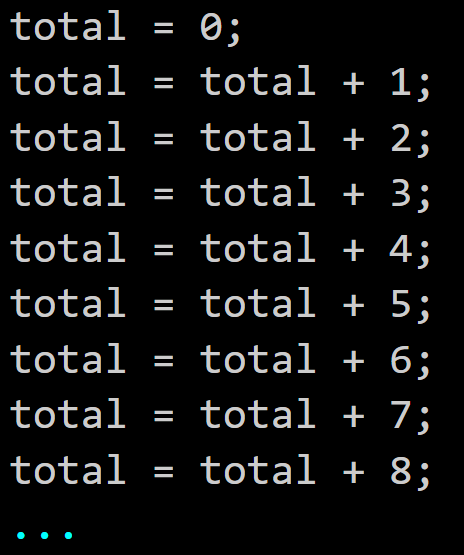
\includegraphics[height = 5cm]{dumbsum.png}}
		\end{center}
		\item<2-> That is repetitive and annoying to read and type out. There has to be a better way.
		\item<3-> This is where loops come into play, they allow us to tell the computer to repeat statements that follow a similar structure.
	\end{itemize}
\end{frame}

%%%%%%%%%%%%%%%%%%%%%%%%%%%%%%%%%%%%%%%%%%%%%%%%%%%%%%%%%

\begin{frame}{For Loops}
	\footnotesize
	\begin{itemize}
		\item Let's look at that sum of the first 17 integers using a \texttt{for} loop
		\begin{center}
			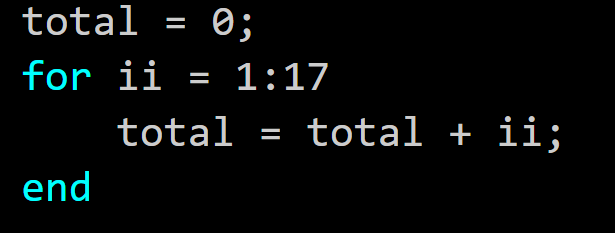
\includegraphics[width = 5cm]{for_example.png}
		\end{center}
		\item<2-> This is much better to look at!
		\item<3-> Let's break down the pieces
		\begin{itemize}
			\item<3-> \texttt{total = 0;} \textbf{initializes} our sum total at 0.
			\item<4-> \texttt{\textcolor{cyan}{for} ii = 1:17} is telling the computer to repeat everything between this line and \texttt{\textcolor{cyan}{end}} for every value of \texttt{ii} starting with \texttt{ii=1} and ending at \texttt{ii=17}. 
			\item<5-> \texttt{total = total + ii;} takes our current value for \texttt{total} and add on our value of \texttt{ii} before stepping to our next \textbf{iteration}, or repeat of the code. 
		\end{itemize}
		\item<6-> Note that we indented the \texttt{total = total + ii;} line to indicate it is a line the loop is repeating.
	\end{itemize}
\end{frame}

%%%%%%%%%%%%%%%%%%%%%%%%%%%%%%%%%%%%%%%%%%%%%%%%%%%%%%%%%

\begin{frame}{While Loops}
	\footnotesize
	\begin{itemize}
		\item Suppose instead we want to find how many numbers to add up before our sum gets greater than 100, this is a task better left for a \texttt{while} loop
		\begin{center}
			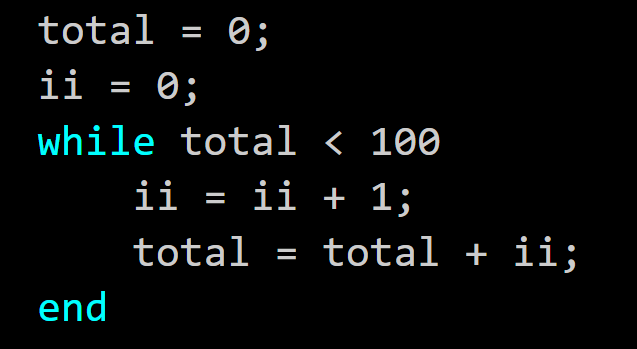
\includegraphics[width = 5cm]{while_example.png}
		\end{center}
		\item<2-> \texttt{\textcolor{cyan}{while} total < 100} tells the computer to repeat the loop while the logical statement \texttt{ total < 100} is true
		\item<3-> In this case we have to update our \textbf{counter} \texttt{ii} ourselves. It helps us count how many times the loop is repeated.
	\end{itemize}
\end{frame}

%%%%%%%%%%%%%%%%%%%%%%%%%%%%%%%%%%%%%%%%%%%%%%%%%%%%%%%%%

\begin{frame}{When to Use Each Loop}
	\footnotesize
	\begin{itemize}
		\item In general, for any loop you need to perform, you could use either a \texttt{for} or \texttt{while} loop. But one is usually preferable based on the context
		\item The general rule of thumb is
		\begin{itemize}
			\item<2-> Use a \texttt{for} loop when you know how many times you need to repeat your loop 
			\item<3-> Use a \texttt{while} loop when you are repeating the loop until some event occurs
		\end{itemize}
	\end{itemize}
	\begin{center}
		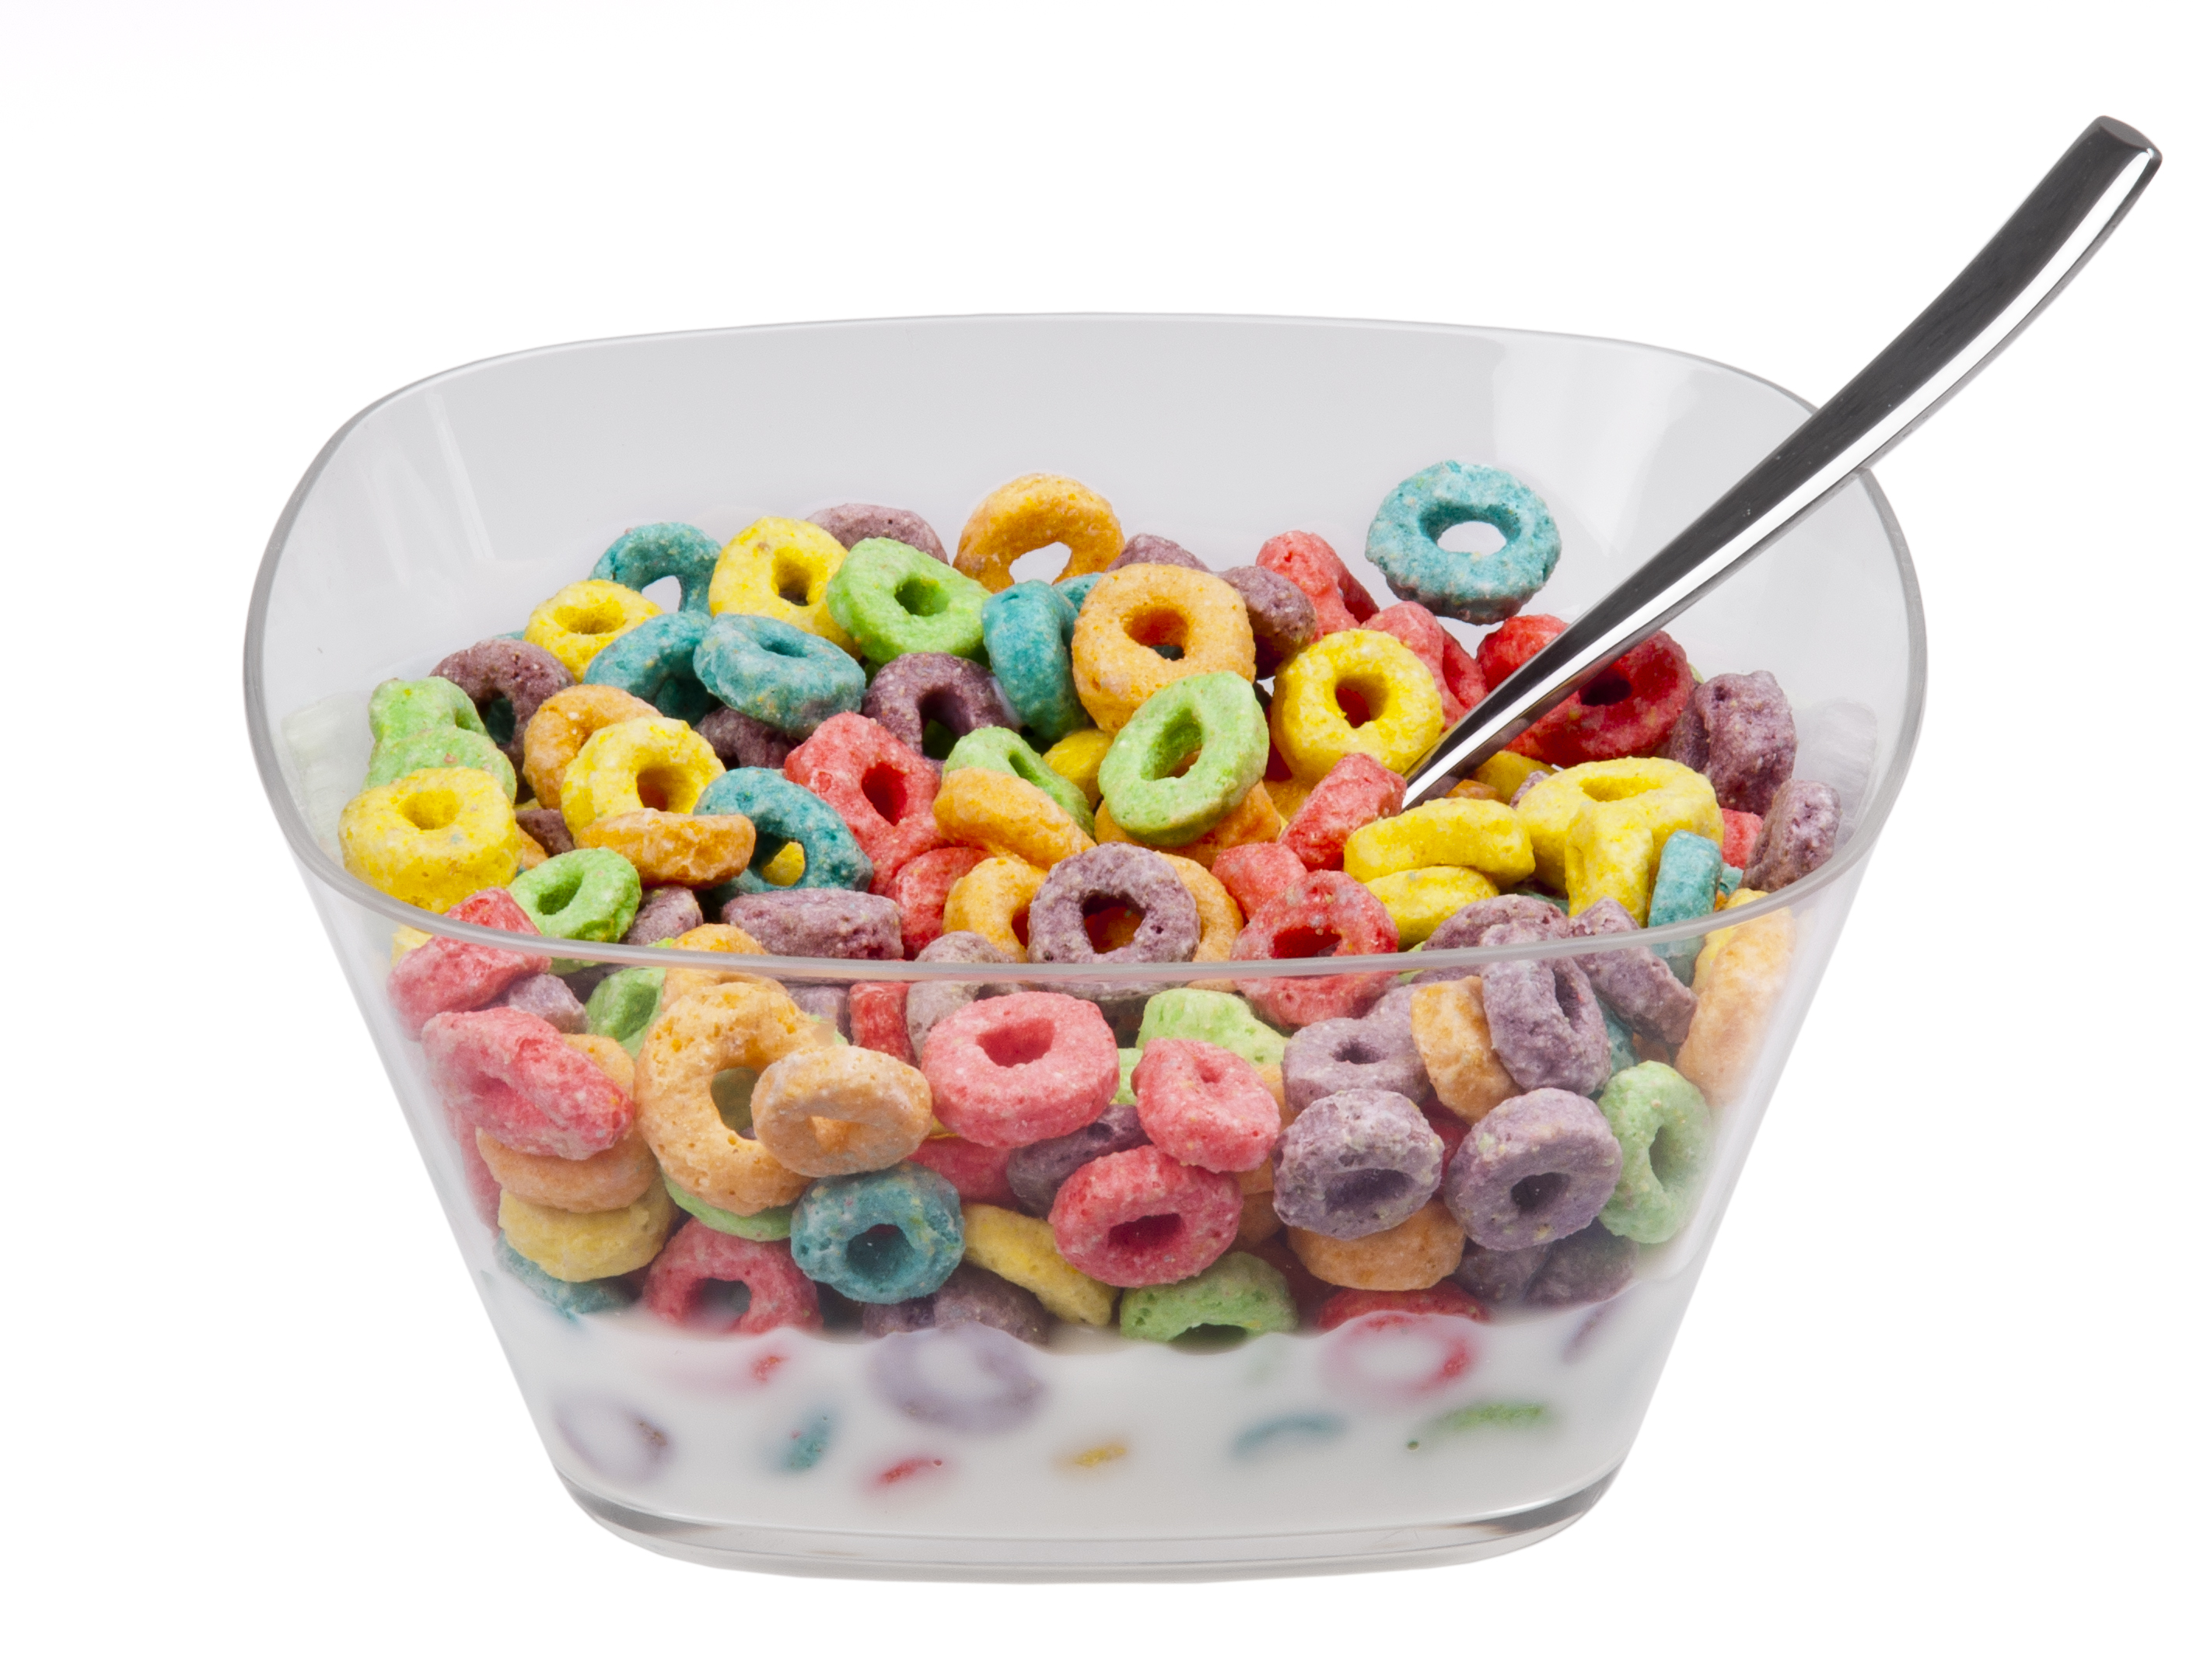
\includegraphics[height = 2.5cm]{Cereal_loops.jpg}
		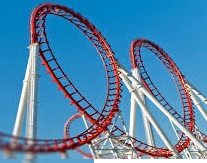
\includegraphics[height = 2.5cm]{Coaster_loops.jpg}
		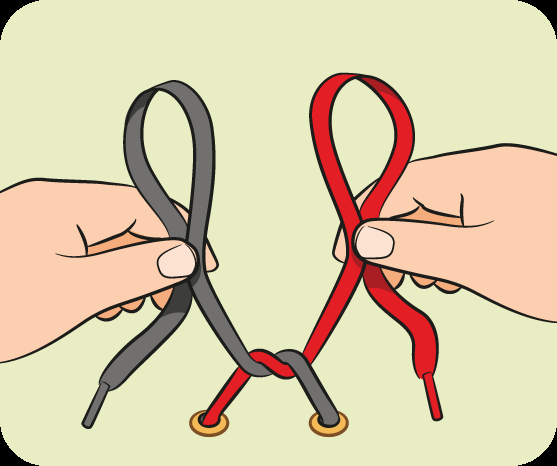
\includegraphics[height = 2.5cm]{shoe_loops.png}
	\end{center}
\end{frame}

%%%%%%%%%%%%%%%%%%%%%%%%%%%%%%%%%%%%%%%%%%%%%%%%%%%%%%%%%
\end{document}